%!TEX program = xelatex
%!TEX root = ./thesis.tex

\section{Hierarchical reinforcement learning methods for multi-modality and sparse environments}
This section will discuss the experiment results on the proposed hierarchical reinforcement learning model.

There are two target tasks to be solved in our experiment setting: "dynamicg8" and "reachcont". The target task "dynamicg8" is a representative problem that has multi-modality state-space, and the target task "reachcont" is a typical problem that has both multi-modality state-space and sparse reward signal. The set of source tasks is  $\{move0, move1, \dots, move7 \}$ for both target tasks.

The problem of hierarchical reinforcement learning consists of two parts: the training of actuator agents and the decider agent. The two problems will be discussed in the following sections.


\subsection{Training the actuator agents with domain randomization by cross-sampling initial states}
As is discussed previously, the learning of the actuator agent of a source task from the source task set is not always the same problem as training a flat reinforcement learning agent for that single task. The initial states generated by actuator agents for other source tasks must be handled, but is usually not encountered in the original source task.

We proposed that the method "domain randomization by cross-sampling initial states" can handle the problem of novel initial states. The performance of this method is experimented in this section. We train the set of source tasks $\{move0, move1, \dots, move7 \}$ simultaneously in this experiment.  

The result is plotted in Figure~\ref{rec_8task_training}, which shows that the actuator agents for some tasks get stuck at sub-optimal scores and fail to solve the corresponding source tasks. As is discussed previously, this problem could be due to the interference between actuator agents.

\begin{figure}[!htbp]
	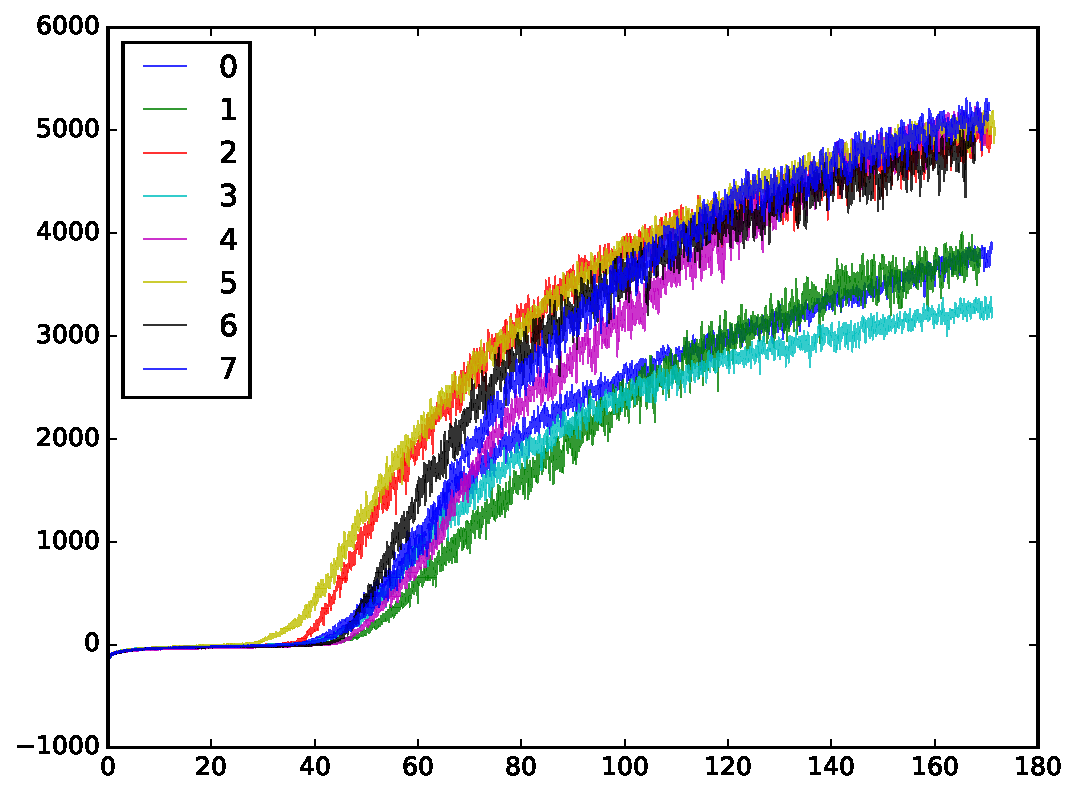
\includegraphics[width=\textwidth]{images/rec_8task_training.pdf}
	\centering
	\caption{Performance of actuator agents with domain randomization by cross-sampling initial states, the x-axis is the number of million time-steps and the y-axis is the total episode reward averaged over the last 200 episodes}\label{rec_8task_training}
\end{figure}

Therefore, we proposed the "synchronous scheduling of actuator learning" method to prevent the learning progress of any actuator agents from lagging behind too far from others. The experiment results of the proposed "synchronous scheduling of actuator learning" is shown in Figure \ref{rec_sync_training}. In this experiments, the policy training of agents who outperforms the global lowest-performance by 1000 is paused until all other actuator agents outperform this agent. The result shows that all the actuator agents reach a final performance of around 6000 although their performance diverge initially. This has verified that the proposed method can successfully prevent the trapped sub-optimal actuator agents. 

\begin{figure}[!htbp]
	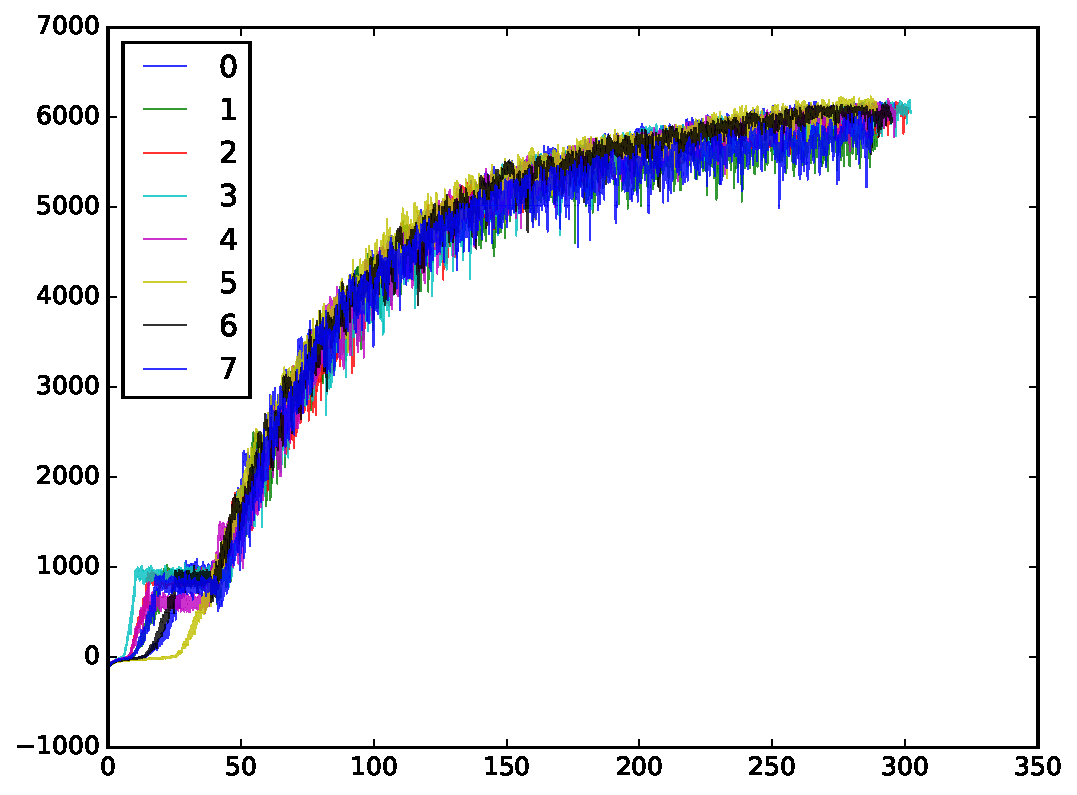
\includegraphics[width=\textwidth]{images/rec_sync_training.pdf}
	\centering
	\caption{Performance of actuator agents using "synchronous scheduling of actuator learning" , the x-axis is the number of million time-steps and the y-axis is the total episode reward averaged over the last 200 episodes}\label{rec_sync_training}
\end{figure}

We consider that the learning of source tasks is successfully solved by the proposed domain randomization by cross-sampling initial states with  synchronous scheduling of actuator learning method.
\subsection{Training the decider agent}
The training of the decider agent consists of two phases: the training of the decision policy and the the switcher policy. We train the two parts in separate phases. In the first phase, the switcher policy is initialized so that it outputs a termination signal whenever the current decision policy has been executed for no less than $l_c$ time steps, which is set to 10 in our experiments. The decision policy is trained with the switcher policy being fixed. After the the performance of the decision policy becomes stable, the switcher policy is then trained with the decision policy fixed.

\subsubsection{Phase 1: Decision policy training}
The performance of the experiment on the training of decision policy on "dynamicg8" is shown in Figure~\ref{fig:rec_dynamicg8_decider_subt10}. The result shows that the agent is able to achieve a reasonable performance of around 2500, while it is not considered optimal.

The performance of the experiment on the training of decision policy on task "reachcont" is shown in Figure~\ref{fig:rec_reachc05_decider_subt10}. The agent achieves a final score of around 0.75 and is considered.


\begin{figure}[!htbp]
\centering
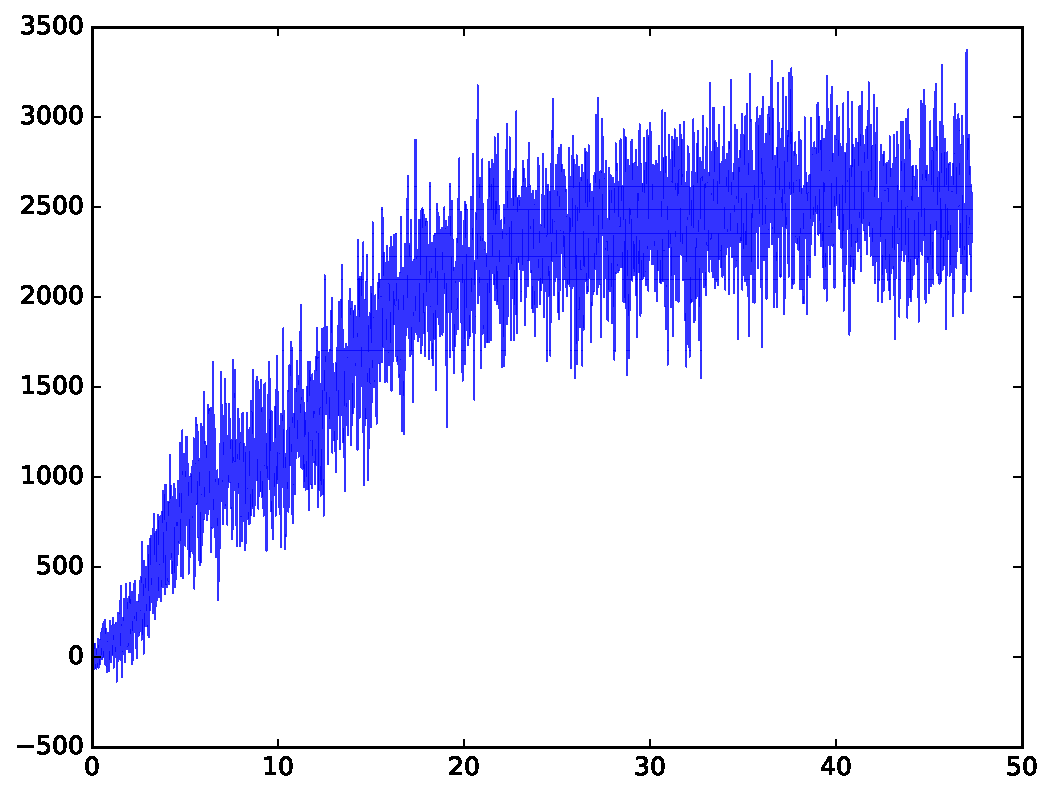
\includegraphics[width=\linewidth]{rec_dynamicg8_decider_subt10}
\caption{Decision policy training performance of the task "dynamicg8", the x-axis is the number of million time-steps and the y-axis is the total episode reward averaged over the last 32 episodes}
\label{fig:rec_dynamicg8_decider_subt10}
\end{figure}


\begin{figure}
\centering
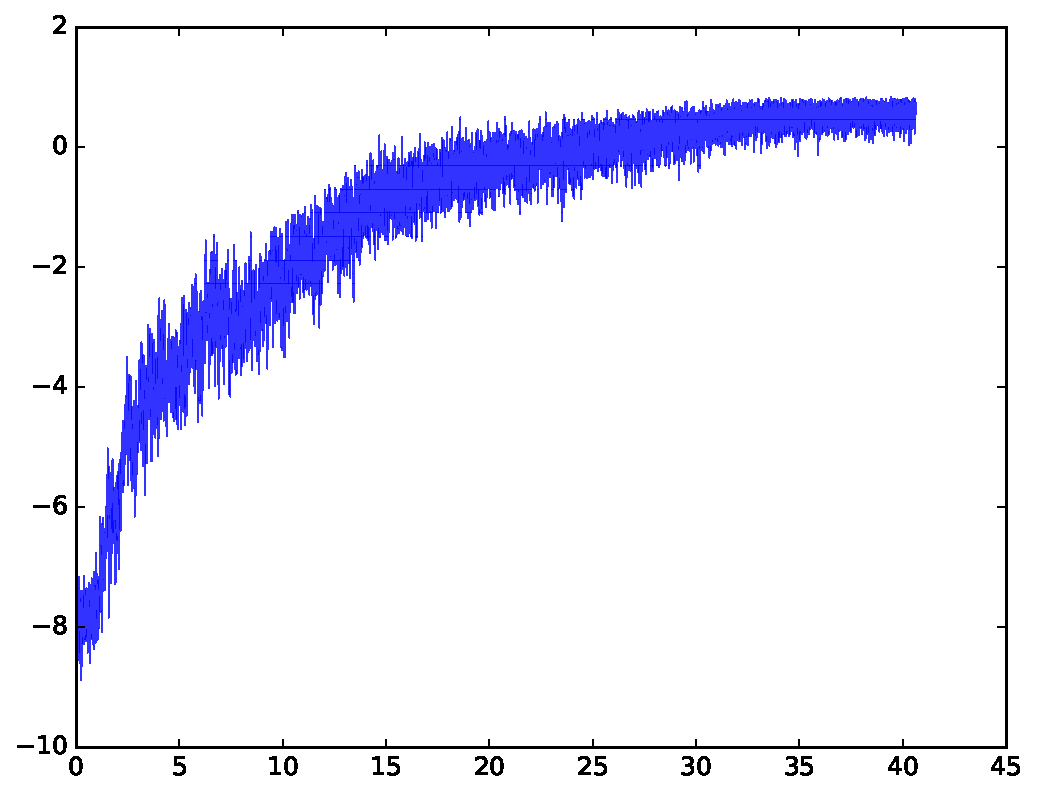
\includegraphics[width=1\linewidth]{rec_reachc05_decider_subt10.pdf}
\caption{Decision policy training performance of the task "reachcont", the x-axis is the number of million time-steps and the y-axis is the total episode reward averaged over the last 200 episodes}
\label{fig:rec_reachc05_decider_subt10}
\end{figure}

The result of the training of the decision policy shows that the hierarchical reinforcement learning agent is able to successfully learn the decision policy. The result is as expected because previous works in SMDP have studied intensively on this problem.

\subsubsection{Phase 2: Switcher policy training}
The parameters of the decision policy is fixed in the second phase of the training, while the switcher policy is trained. The switcher policy is re-initialized randomly at the beginning of this phase, so that it outputs a termination signal with a probability around 0.5. This reinitialized switcher policy is different from the switcher policy in phase 1, which outputs a termination signal deterministically after the current actuator policy has been executed for a pre-defined number of steps.

The reinforcement learning performance during the training of switcher policy on the task "dynamicg8" is shown in Figure~\ref{fig:rec_dynamicg8_switcher}. The decider agent appears to achieve a relatively stable performance during the training of the switcher policy, without any significant degradation from the final performance of phase 1.

The average execution length of the decision policies is plotted in Figure~\ref{fig:rec_dynamicg8_avesubt}. The agent manages to find a better switcher policy since the final average execution length becomes around $10$ while it was around $5$ in phase 1. As the result, the decision policy does not need to compute its output as frequently as in phase 1.

Therefore, the training of switcher policy as considered to be useful on the task "dynamicg8", in the sense that the agent can maintain a good performance as well as minimize the number of decisions being made by the decider agent. 
\begin{figure}[!htbp]
	\centering
	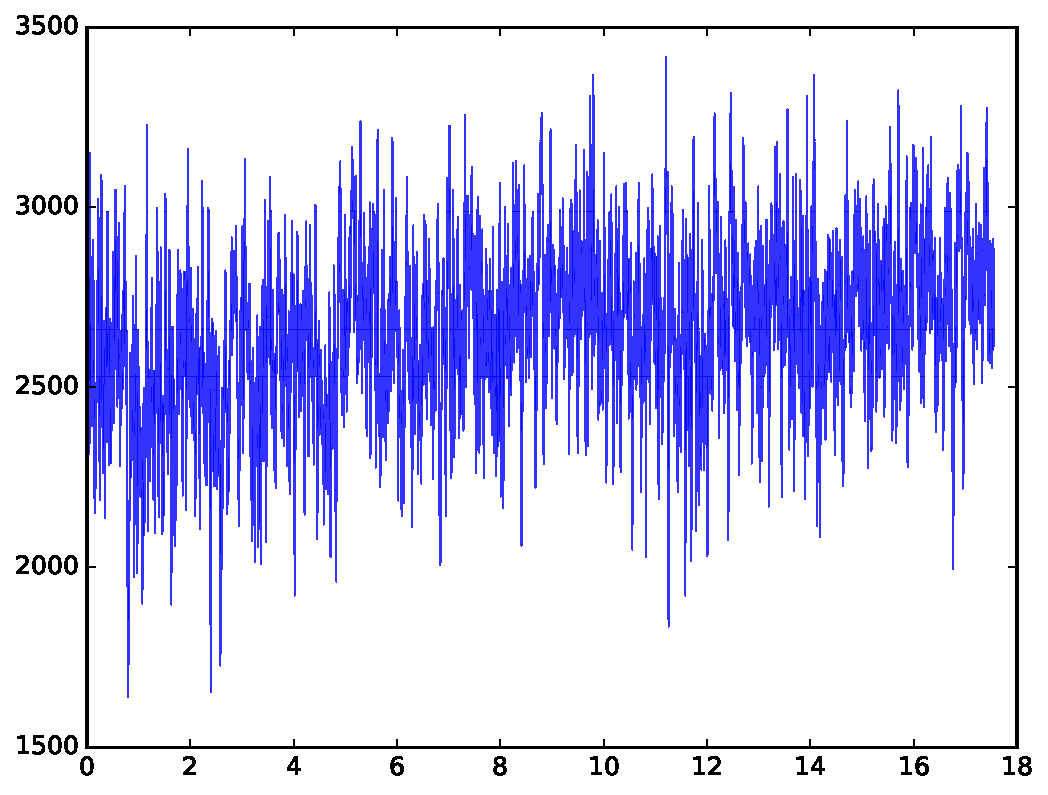
\includegraphics[width=\linewidth]{rec_dynamicg8_switcher}
	\caption{Switcher policy training performance of the task "dynamicg8", the x-axis is the number of million time-steps and the y-axis is the total episode reward averaged over the last 32 episodes}
	\label{fig:rec_dynamicg8_switcher}
\end{figure}

\begin{figure}[!htbp]
	\centering
	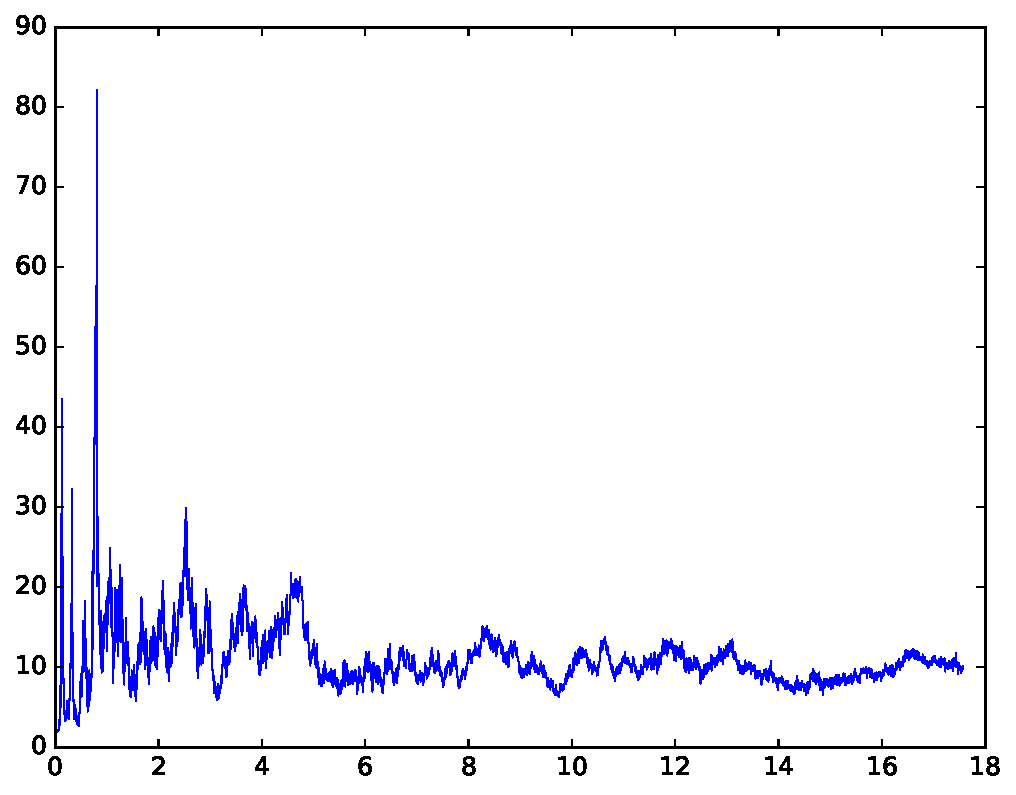
\includegraphics[width=\linewidth]{rec_dynamicg8_avesubt}
	\caption{Average execution length of the actions of decision policies of the task "dynamicg8", the x-axis is the number of million time-steps and the y-axis is the decision policy's average execution length of the last batch.}
	\label{fig:rec_dynamicg8_avesubt}
\end{figure}

The reinforcement learning performance during the training of switcher policy on the task "dynamicg8" is shown in Figure~\ref{fig:rec_reachcont_switcher}. The final performance has been improved from $0.75$ in the decision policy training to around $0.81$. The training of switcher policy appears to beneficial to the performance of the target task.

The average execution length of the decision policies is plotted in Figure~\ref{fig:rec_dynamicg8_avesubt}. The final average value of the execution length appears to be reduced to $1.6$, compared to $5$ in the decision policy training phase.

Therefore, the switcher policy is able to improve the reinforcement learning performance at the expense of the computation spent on the decision policy being increased.

\begin{figure}[!htbp]
	\centering
	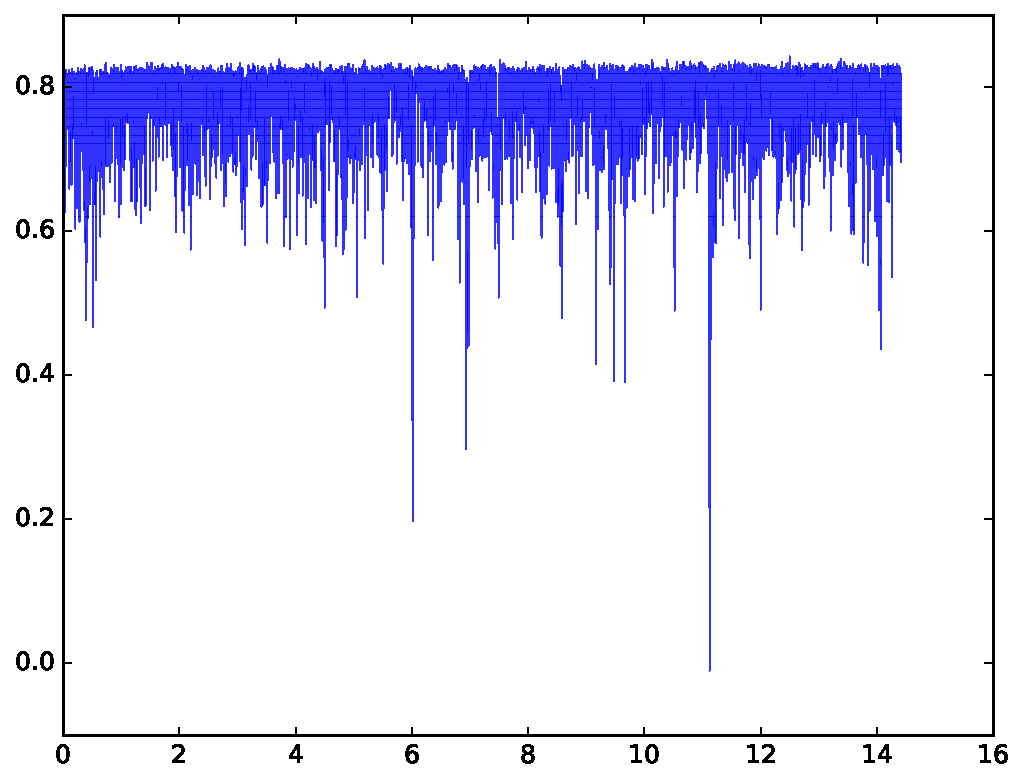
\includegraphics[width=\linewidth]{rec_reachcont_switcher}
	\caption{Switcher policy training performance of the task "reachcont", the x-axis is the number of million time-steps and the y-axis is the total episode reward averaged over the last 32 episodes}
	\label{fig:rec_reachcont_switcher}
\end{figure}

\begin{figure}[!htbp]
	\centering
	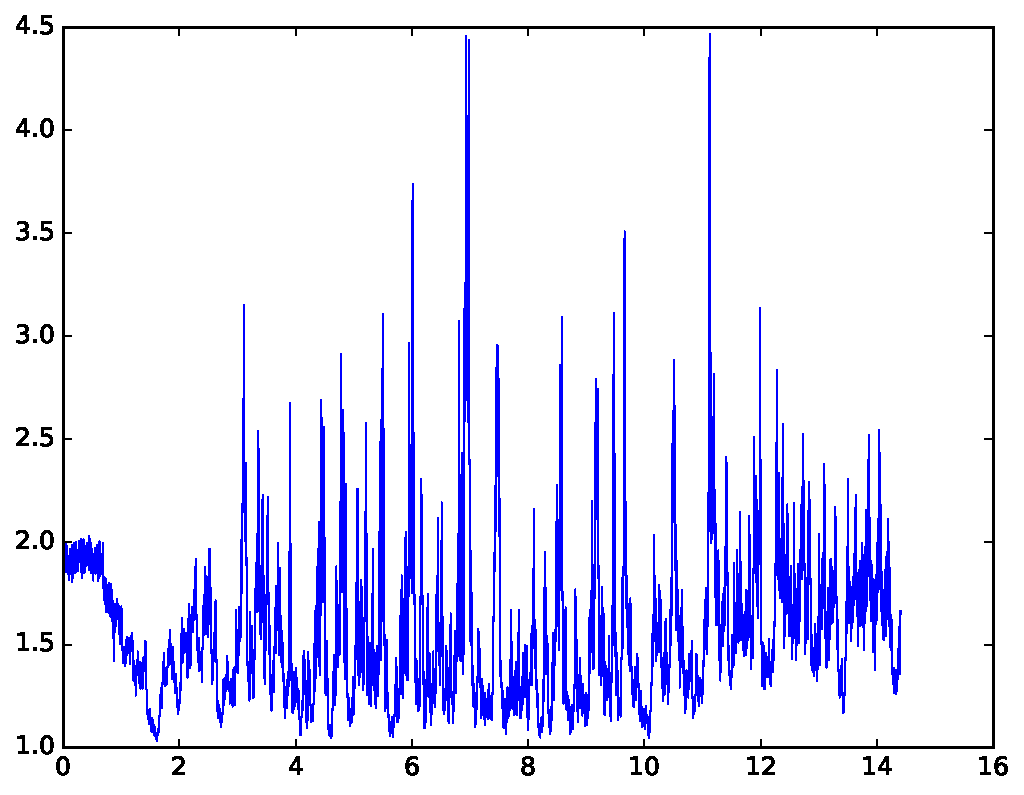
\includegraphics[width=\linewidth]{rec_reachcont_switcher_subt}
	\caption{Average execution length of the actions of decision policies of the task "reachcont", the x-axis is the number of million time-steps and the y-axis is the decision policy's average execution length of the last batch.}
	\label{fig:rec_reachcont_switcher_subt}
\end{figure}